\documentclass{article} 
\usepackage{tcolorbox}
\usepackage{alltt, fancyvrb, url}
\usepackage{graphicx}
\usepackage[utf8]{inputenc}
\usepackage{float}
\usepackage{hyperref}
\usepackage{amsthm}
\newtheorem{definition}{Definition}
% Questo commentalo se vuoi scrivere in inglese.
\usepackage[italian]{babel}
\usepackage[italian]{cleveref}

\tcbuselibrary{skins}

\usepackage{background}
\SetBgHshift{-2.3cm}
\SetBgVshift{0cm}

\usepackage[margin=3cm]{geometry}

\usepackage{tikz}
\usepackage{tikzpagenodes}


\usepackage{xparse}
\DeclareDocumentCommand\topic{ m m g g g g g}
{
\begin{tcolorbox}[sidebyside,sidebyside align=top,opacityframe=0,opacityback=0,opacitybacktitle=0, opacitytext=1,lefthand width=.3\textwidth]
\begin{tcolorbox}[colback=red!05,colframe=red!25,sidebyside align=top,width=\textwidth,before skip=0pt]
#1.\end{tcolorbox}%
\tcblower
\begin{tcolorbox}[colback=blue!05,colframe=blue!10,width=\textwidth,before skip=0pt]
#2
\end{tcolorbox}
\IfNoValueF {#3}{
\begin{tcolorbox}[colback=blue!05,colframe=blue!10,width=\textwidth]
#3
\end{tcolorbox}
}
\IfNoValueF {#4}{
\begin{tcolorbox}[colback=blue!05,colframe=blue!10,width=\textwidth]
#4
\end{tcolorbox}
}
\IfNoValueF {#5}{
\begin{tcolorbox}[colback=blue!05,colframe=blue!10,width=\textwidth]
#5
\end{tcolorbox}
}
\IfNoValueF {#6}{
\begin{tcolorbox}[colback=blue!05,colframe=blue!10,width=\textwidth]
#6
\end{tcolorbox}
}
\IfNoValueF {#7}{
\begin{tcolorbox}[colback=blue!05,colframe=blue!10,width=\textwidth]
#7
\end{tcolorbox}
}
\end{tcolorbox}
}

\def\summary#1{
\begin{tikzpicture}[overlay,remember picture,inner sep=0pt, outer sep=0pt]
\node[anchor=south,yshift=-1ex] at (current page text area.south) {% 
\begin{minipage}{\textwidth}%%%%
\begin{tcolorbox}[colframe=white,opacityback=0]
\begin{tcolorbox}[enhanced,colframe=black,fonttitle=\large\bfseries\sffamily,sidebyside=true, nobeforeafter,before=\vfil,after=\vfil,colupper=black,sidebyside align=top, lefthand width=.95\textwidth,opacitybacktitle=1, opacitytext=1,
segmentation style={black!55,solid,opacity=0,line width=3pt},
title=Summary
]
#1
\end{tcolorbox}
\end{tcolorbox}
\end{minipage}
};
\end{tikzpicture}
}

\usepackage{listings}
\usepackage{color}

\definecolor{dkgreen}{rgb}{0,0.6,0}
\definecolor{gray}{rgb}{0.5,0.5,0.5}
\definecolor{mauve}{rgb}{0.58,0,0.82}

\lstset{frame=tb,
  language=Python,
  aboveskip=3mm,
  belowskip=3mm,
  showstringspaces=false,
  columns=flexible,
  basicstyle={\small\ttfamily},
  numbers=none,
  numberstyle=\tiny\color{gray},
  keywordstyle=\color{blue},
  commentstyle=\color{dkgreen},
  stringstyle=\color{mauve},
  breaklines=true,
  breakatwhitespace=true,
  tabsize=3,
  numbers=left
}

% Intestazione degli appunti
\author{Andrea Cecchini}
\title{\textbf{Metodi Numerici per \\ L'intelligenza Artificiale.}}
\date{\today}
% Inizio del documento
\begin{document}
\maketitle
\newpage
\tableofcontents
\newpage
% Section: Introduzione all'Analisi Numerica.
\section{Introduzione all'Analisi Numerica.}
\subsection{Analisi Numerica.}
Introduciamo nel definire il compito dell'analisi numerica.
%
\topic{\textbf{Analisi Numerica}}
{
    L'Analisi Numerica è la parte di matematica 
    %
    che si occupa di dare una \textbf{risposta numerica} 
    %
    ad un problema matematico  che modellizza un problema reale.    
}
\subsubsection{Fasi della risoluzione di un problema numerico.}
%
Al fine di raggiungere tale problema, ci avvaliamo delle seguenti fasi:
%
\begin{itemize}
    \item \textbf{Tradurre} il problema reale in un insieme di equazioni 
%
    matematiche in grado di descriverlo
    \item \textbf{Trasformare} il problema matematica nel continuo in un 
%
    problema numerico discreto che sia risolubile.
    \item \textbf{Trasportare}  il problema discreto in un calcolatore mediante 
%
    l’applicazione di algoritmi numerici capaci di determinare la soluzione 
%
    in un tempo ottimale.
    \item \textbf{Interpretare} la soluzione numerica nei termini 
%
    della situazione reale e \textbf{verificare} così sia l’adeguatezza del modello 
%
    matematico sia l’efficienza dell’algoritmo risolutivo.
\end{itemize}
\subsubsection{Errori nel risolvere un problema numerico.}
Nel percorso appena descritto vi possono essere numerevoli errori, 
%
le quali sorgenti sono:
\begin{itemize}
    \item \textbf{Errori nel modello matematico} Nascono da una cattiva 
%
    traduzione del problema reale a quello matematico, per esempio si 
%
    considerano alcune cose come trascurabili quando non lo sono.
    \item \textbf{Errori nel modello numerico-computazionale} Vengono 
%
    descritti come errori di \textit{discretizzazione} o \textit{troncamento}.
    \item \textbf{Errori presenti nei dati} Nati da uno strumento di
%
    misurazione fallace o da misurazioni che possono essere influenzate
%
    da errori sistematici.
    \item \textbf{Errori di arrotondamento nei dati e nei calcoli} Sono 
%
    gli errori introdotti nella rappresentazone dei numeri sul calcolatore.
\end{itemize}
\newpage
\subsection{Classificazione dei problemi numerici}
\subsubsection{Problema numerico}
\topic{\textbf{Problema Numerico}}
{
    Per \textbf{problema numerico}
    %
        intendiamo una descrizione chiara di una \textbf{relazione funzionale}  
    %
        tra i dati (\textbf{input}) e i risultati (\textbf{output}).   
}
In particolare, in un problema numerico abbiamo i seguenti elementi:
\begin{itemize}
    \item \textbf{F} rappresenta la relazione funzionale tra input ed output.
    \item \textbf{x} rappresenta il dato di input della relazione funzionale.
    \item \textbf{y} rappresenta l’output dell<a funzione di un determinato input
\end{itemize}
\subsubsection{Classificazione dei problemi numerici.} Descritti questi 
%
3 elementi, è possibile classificare il problema numerico in base a 
%
cosa stiamo cercando:
\begin{itemize}
    \item \textbf{Problema diretto} \textbf{F} e \textbf{x} sono dati,
%
    bisogna \textbf{trovare y}.
    \item \textbf{Problema inverso} \textbf{F} e \textbf{y} sono dati,
%
    bisogna \textbf{trovare x}.
    \item \textbf{Problema di identificazione} \textbf{x} e \textbf{y} sono noti,
%
    bisogna trovare \textbf{F}.
\end{itemize}
Quest’ultimo problema è quello che interesserà di più durante il corso, 
%
perchè è proprio il problema numerico che l’intelligenza artificiale
%
cerca di risolvere.

\summary{
    Abbiamo introdotto la materia dell'\textbf{analisi numerica}
%
    e quello che si prefissa di risolvere.
%
    Successivamente abbiamo definito il concetto di 
%    
    \textbf{problema numerico} ed abbiamo elencato i diversi tipi,
%
    quali \textbf{problema diretto}, \textbf{problema inverso} e
%
    \textbf{problema di identificazione}.
}
% End Section: Introduzione all'Analisi Numerica.
\newpage
\section{Introduzione all'Intelligenza artificiale}
\topic{\textbf{Intelligenza Artificiale}}
{
    Per \textbf{intelligenza artificiale} si intende una parziale 
%
    riproduzione dell'attività intellettuale propria dell'uomo.
}
Esistono due tipi di intelligenze artificiali, basate sul loro 
%
dominio applicativo:
\begin{itemize}
    \item \textbf{Intelligenza artificiale ``debole``}:
    Sono dei sistemi basati per risolvere \textbf{problemi specifici.}
    \item \textbf{Intelligenza artificiale ``forte``}:
    Sono dei sistemi in grado di replicare \textbf{tutte le funzioni cognitive}
%
    dell'essere umano. Spesso per riferirci a questa categoria useremo il termine
%
    \textbf{``Intelligenza Generalista``}.
\end{itemize}
Molti tendono a confondere e a non capire il legame tra \textbf{intelligenza artificiale},
%
,\textbf{machine learning} e \textbf{deep learning}.
\\
Rappresenteremo il loro legame attraverso il seguente diagramma di Venn:
\begin{center}
    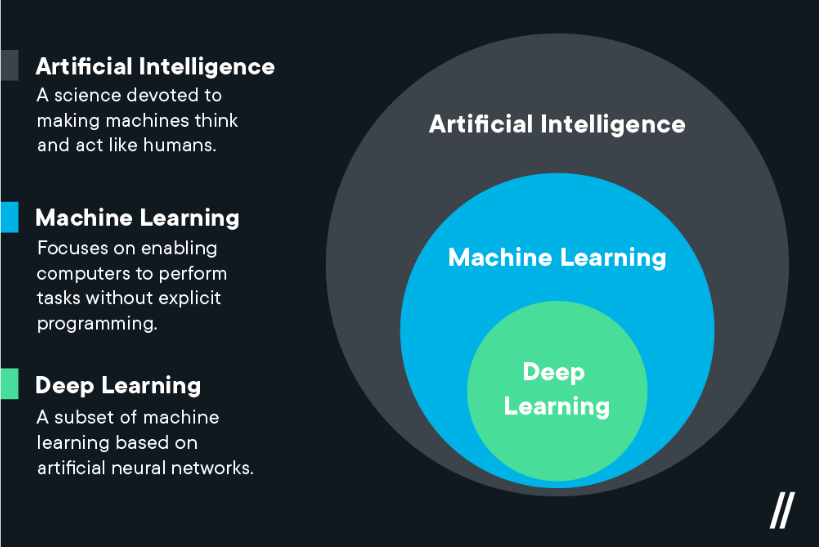
\includegraphics[scale=0.7]{images/AI_ML_DL.png}
\end{center}
Detto ciò, capiamo cosa cambia grazie all'utilizzo di questa tecnologia.
\subsection{Cambio di paradigma di programmazione}
\subsubsection{Paradigma classico}
\begin{center}
    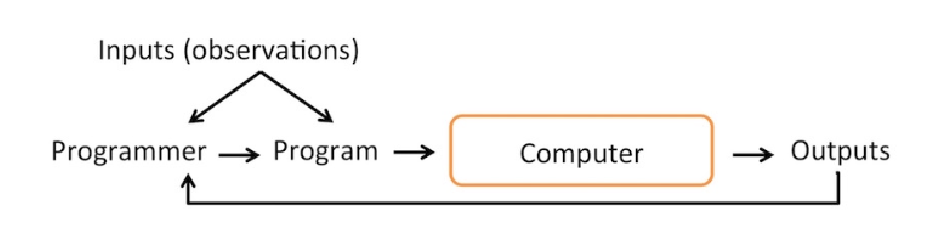
\includegraphics[scale=0.7]{images/Paradigma_Classico.png}
\end{center}
Il paradigma sul quale noi siamo abituare a creare programmi è
%
il seguente:
\begin{itemize}
    \item Il \textbf{programmatore} elabora e crea un 
%   
    \textbf{algoritmo} (programma).
    \item All'algoritmo vengono forniti dei dati come \textbf{input}.
    \item L'elaboratore computa l'input sulla base dell'algoritmo
%
    e fornisce un output.
\end{itemize}
Questo modo di agire prevede una forte presenza dell'essere umano,
%
il quale in veste di programmatore, crea l'algoritmo voluto. 
\subsubsection{Paradigma del Machine Learning}
\begin{center}
    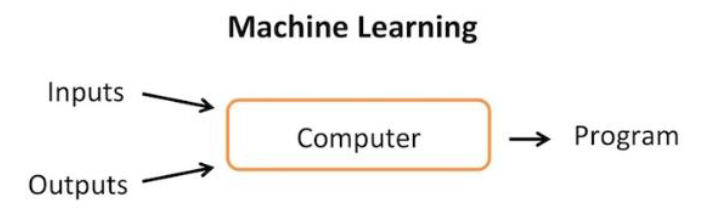
\includegraphics[scale=0.7]{images/Paradigma_del_ML.png}
\end{center}
In questo paradigma il ruolo dell'uomo viene ``sostituito'' dalla
%
tecnica del \textbf{Machine Learning}.
\topic{Machine Learning}
{
    Sistema in grado di apprendere automaticamente da esempi 
%
    specifici (\textbf{training data}) e di generalizzare la 
%
    conoscenza su nuovi campioni (\textbf{test data}) dello stesso
%
    dominio
}
Difatti, il machine learning dato input ed output, procede nella
%
risoluzione del problema di identificazione.
\\
Andiamo ad analizzare le diverse fasi di questo paradigma:
\\  
\begin{center}
    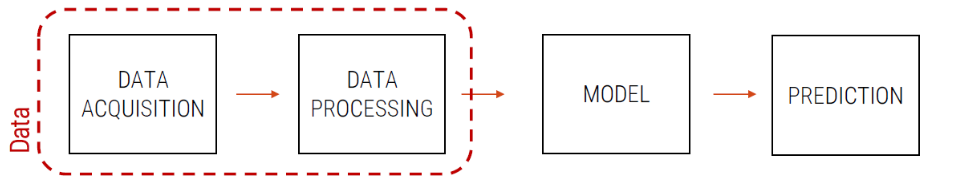
\includegraphics[scale=0.7]{images/Paradigma_ML_fasi.png}
\end{center}
\begin{itemize}
    \item \textbf{Acquisizione dati} I dati sono l'elemento base
%
    di tutte le applicazioni di M.L.. E' molto importante quindi
    sapere come acquisire questi dati.
    \item \textbf{Data processing} I dati raccolti nella fase 
%
    precedente vengono processati al fine da attarli al meglio al 
%
    al modello M.L. che intendiamo sviluppare.
    \item \textbf{Modello} Insieme di techiche matematiche e 
%
    statistiche in grado di apprendere da una certa distribuzione di 
%
    dati.
    \item\textbf{Predizione} Una volta ottenuto il modello è 
% 
    possibile ``predire'' l'output correlato ad un certo input non 
%
    presentato nel training data.
\end{itemize}
\newpage
\subsection{I dati}
\subsubsection{Acquisizione dei dati}
E' possibile ottenere i dati in due modi:
\begin{itemize}
    \item Usare set di dati pubblici: sono presenti molte
%
    piattaforme, come \href{https://www.kaggle.com/datasets}{kaggle}.
    \item Acquisento un nuovo set di dati.
\end{itemize}
E' molto  comune nel mondo della ricerca di fornire questi set di 
%
dati pubblici, in modo altruista.
\\
Visto ciò, non usarli sarebbe un peccato.
\subsubsection{Annotazione dei dati}
\topic{Etichetta}
{
    Annotare i dati vuol dire assegnare un \textbf{etichetta} 
%    
    (output) ad una determinata istanza di input.
%
    L'etichetta rappresenta il contenuto semantico dei dati.
}
Diremo quindi che un dato è \textbf{annotato} se associato ad una 
%
\textbf{etichetta}.
\\
I dati non annotati sono spesso \textbf{inutili}.
Tuttavia, grazie alla tecnica di apprendimento 
%
\textbf{non supervisionata} (vedremo dopo) è possibile comunque 
%
estrarre conoscenza da essi.
\subsubsection{Organizzazione dei dati}
Bisogna \textbf{organizzare} i dati come segue: 
\begin{itemize}
    \item \textbf{Training set} sono i dati sui quali il modello 
%
    apprende automaticamente durante la fase di apprendimento.
    \item \textbf{Validation set} sottoinsieme del training set, 
%
    sono i dati con il quali si informa il sistema della 
%
    validazione del suo apprendimento.
    \item \textbf{Testing set} dati con il quali si testa il 
%
    modello. Questa fase verifica l'efficacia del modello, anche
%
    attraverso misure numberiche qualitative e quantitative.
\end{itemize}
\begin{center}
    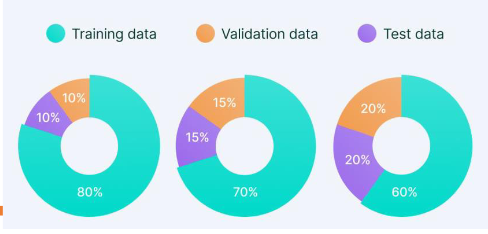
\includegraphics[scale=0.7]{images/Organizzazione_dei_dati.png}
\end{center}
Nell'immagine qui sopra si elenca differenti proporzioni in cui 
%
si dovrebbe suddividere il set di dati che abbiamo nei subset 
%
descritti precedentemente.
\subsection{Complessità dei dati}
\topic{\textbf{Dimensionalità}}
{
    La \textbf{dimensionalità} di un dato rappresenta la 
%
    \textbf{densità} di quest'ultimo, ovvero la quantità.
}
\topic{\textbf{Complessità}} 
{
    Diremo che un dato è complesso se presenta una 
%
    \textbf{alta dimensionalità}. 
}
Dare al sistema di M.L. una mole spoporzionata di dati, come tutti
%
i pixel di un'immagine, non è una buona cosa.
\\
Se stessimo lavorando su un classificatore di immagini, sarebbe un
%
errore grave dargli dati ad alta dimensionalità, in quanto non 
%
riuscirebbe ad apprendere da così tanti dati \textbf{inutili}.
\\ 
La soluzione a questo problema si chiama \textbf{feature extraction}.
\begin{center}
    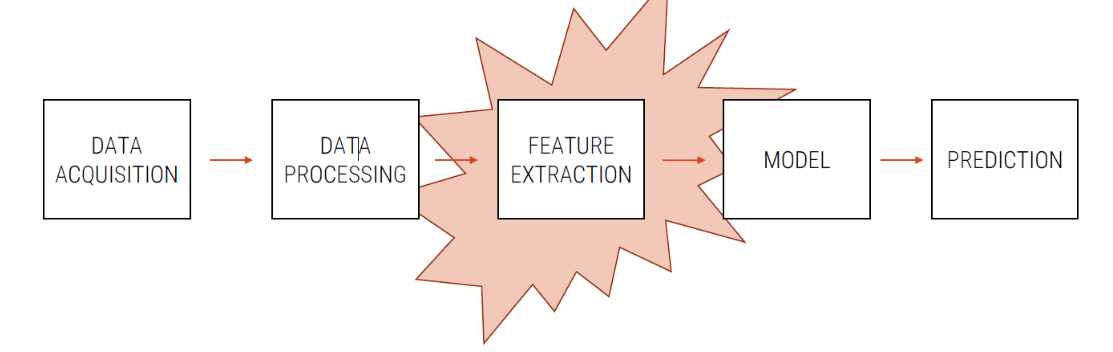
\includegraphics[scale=0.5]{images/Feature_extraction.png}
\end{center}
\subsubsection{Feature extraction}
\topic{\textbf{Feature}}
{
    La \textbf{feature} srappresenta la parte più utile del dato 
%
    grezzo.
}
\topic{\textbf{Feature Expansion}}
{
    Rappresenta l'operazione di estrazione di features dal dato grezzo.
\\ 
    E' un modo per creare un nuovo e più piccolo insieme di dati 
%
    che cattura la maggiore parte dell'informazione dei dati grezzi.
}
\topic{\textbf{Feature Descriptor}}
{
    Un \textbf{featuer descriptor} rappresenta un vettore \(n\)
%
    dimensionale di feature numeriche che rappersentano qualche
%
    oggetto.
}
\begin{center}
    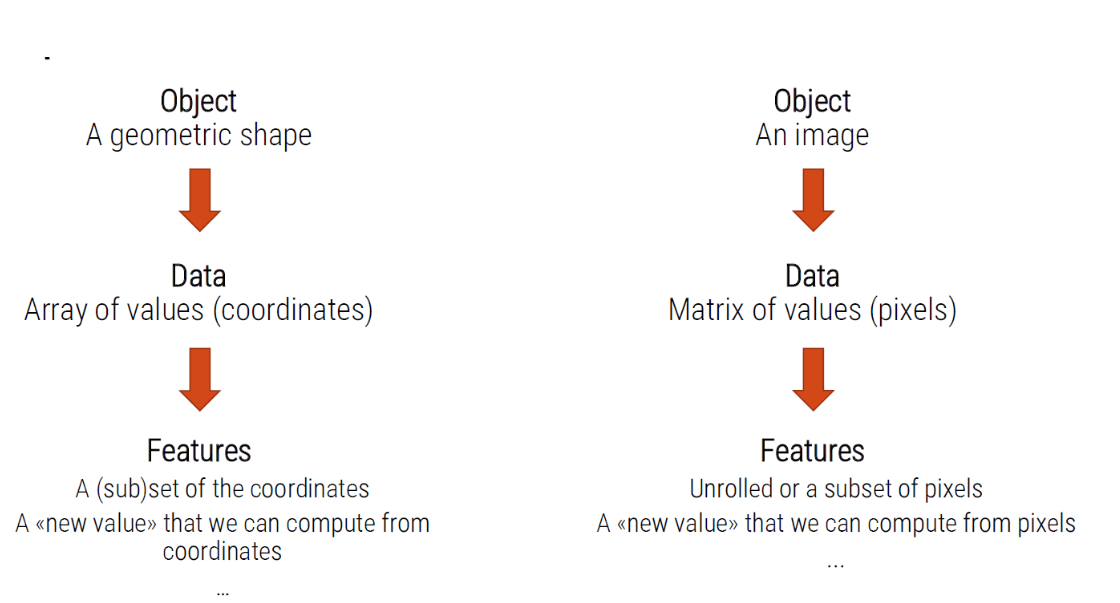
\includegraphics[scale=0.5]{images/Feature_example.png}
\end{center}
\newpage
\subsection{Machine Learning tasks}
Il machine learning offre diversi \textbf{task} a seconda dell'output
%
che vogliamo
\begin{itemize}
    \item \textbf{Classificazione}
    \item \textbf{Regressione}
    \item \textbf{Clustering}
\end{itemize}
\subsubsection{Classificazione}
\topic{\textbf{Classe}}
{
    Una classe è un \textbf{set di dati con proprietà comuni}.
\\ 
    Il concetto di classe è correlato al concetto di ``etichetta''.
}
\topic{\textbf{Classificazione}}
{
    Dato un input specifico, il modello (\textbf{classificatore})
%
    emette una \textbf{classe}.
}
\begin{itemize}
    \item Se ci sono 2 classi, chiamiamo il problema come 
%    
    \textbf{problema di classificazione binaria}
    \item Se ci sono \( n \) classi con \( n > 2\), chiamiamo il 
%
    problema come \textbf{problema di classificazione multiclasse}.
\end{itemize}
\subsubsection{Regressione}
\topic{\textbf{Regressione}}
{
    La \textbf{relazione} viene utilizzata per \textbf{modellare la 
%    
    relazione} tra le variabili indipendenti e le variabili dipendenti. 
}
Quindi la regressione si occupa di risolvere un \textbf{problema
%
di identificazione}.
\topic{\textbf{Regressione MultiVariata}}
{
    La \textbf{regressione multivariata} prevede l'impiego di più
%
    variabili in gioco rispetto alla classica regressione lineare.
}
\newpage
\subsubsection{Clustering}
\topic{\textbf{Clustering}}
{
    Il \textbf{clustering} permette di identificare dei gruppi
%
    di dati in classi, senza saper a priori le classi.
}
Il clustering è spesso applicato, infatti, in un ambiente di 
%
apprendimento non supervisionato, in cui le classi del problema
%
non sono noti a priori.
% Aggiungere immagini
\subsection{Loss Function}
Facciamo una picolissima diramazione di poche righe per spiegare 
%
il concetto di \textbf{loss function}.
\topic{\textbf{Loss Function}}
{
    La \textbf{loss function} (funzione di perdita) è un indicatore
%
    che permette di descrivere la  qualità dell'apprendimento del 
%
    sistema.
}
Al fine di aver un sistema che appreso in maniera esaustiva, 
%
bisogna far tendere verso il basso il valore della \textbf{loss 
%
function}.
\subsection{Tipi di apprendimento}
\subsubsection{Apprendimento supervisionato}
\subsubsection{Apprendimento non supervisionato}
\subsubsection{Apprendimento con rinforzo}
\end{document}
 